%ekg_7_Realisierung/Diskussion der Alternativen

\subsection{Konzeptfindung und Diskussion der Alternativen}

Dieses Unterkapitel führt die Anforderungen und die gewählten Lösungen auf, ohne diese im Detail zu erklären. Die genaue Erläuterung der verfolgten und getesteten Umsetzungen sind Inhalt der folgenden Kapitel der Realisierung. Ebenso werden hier die Lösungen aufgeführt, die sich nach dem Test als zu ineffizient oder zu aufwendig für die Anwendung erwiesen haben.

\subsubsection{Konzeptionierung}

Zur Erstellung eines Konzeptes für das EKG-Gerät wurden zunächst alle Anforderungen die sich aus dem Signal und den Produktvorstellungen ergaben, gesammelt. Hierzu zählen auch Funktionen die über die bloße Aufzeichnung eines EKGs hinausgehen.

\begin{enumerate}
\item Bandbreite der Filterschaltung: \SI{0.5}{\hertz} - \SI{150}{\hertz}
\item Abtastfrequenz: \SI{250}{\hertz} - \SI{1000}{\hertz}
\item Benötigte Verstärkung für das EKG-Signals: \SI{66}{\decibel} (= Faktor 2000)
\item Für ein Ein-Kanal-EKG muss eine Differenzbildung der Signale zwischen den beiden Ableitungspunkten durchgeführt werden
\item Die negativen Signalanteile des EKGs müssen mit einer unipolaren Versorgungsspannung übertragen werden
\item Durch Magnetfelder von umgebenden Versorgungsleitungen induzierte Störsignale (sogenanntes Netzbrummen) müssen unterdrückt werden
\item Die verwendeten aktiven elektronischen Bauteile müssen mit einer unipolaren Versorgungsspannung betrieben werden können und sollten diesen Spannungsbereich fast vollständig ausnutzen
\item Zur Anzeige des Signals soll wahlweise ein integriertes Display oder das eigene Smartphone verwendet werden
\item Die Bedienung erfolgt via Touchscreen mit einem intuitiven User-Interface
\item Als Aufnahmemodi werden ein Kurzzeit-EKG (\SI{2}{\min}) und ein Langzeit-EKG (24 Stunden) angeboten
\item Die Betriebslaufzeit muss mindestens 30 Stunden betragen
\item Die Energieversorgung erfolgt über einen Lithium-Ionen-Akku
\item Die aufgenommenen Daten werden auf einem externen Speichermedium gesichert
\item Bei einem niedrigen Akkustatus soll das Gerät den Nutzer durch einen akustischen Warnton darauf hinweisen
\end{enumerate}

%TODO Konzept der Filterung

\begin{figure} [h]
	%\centering
	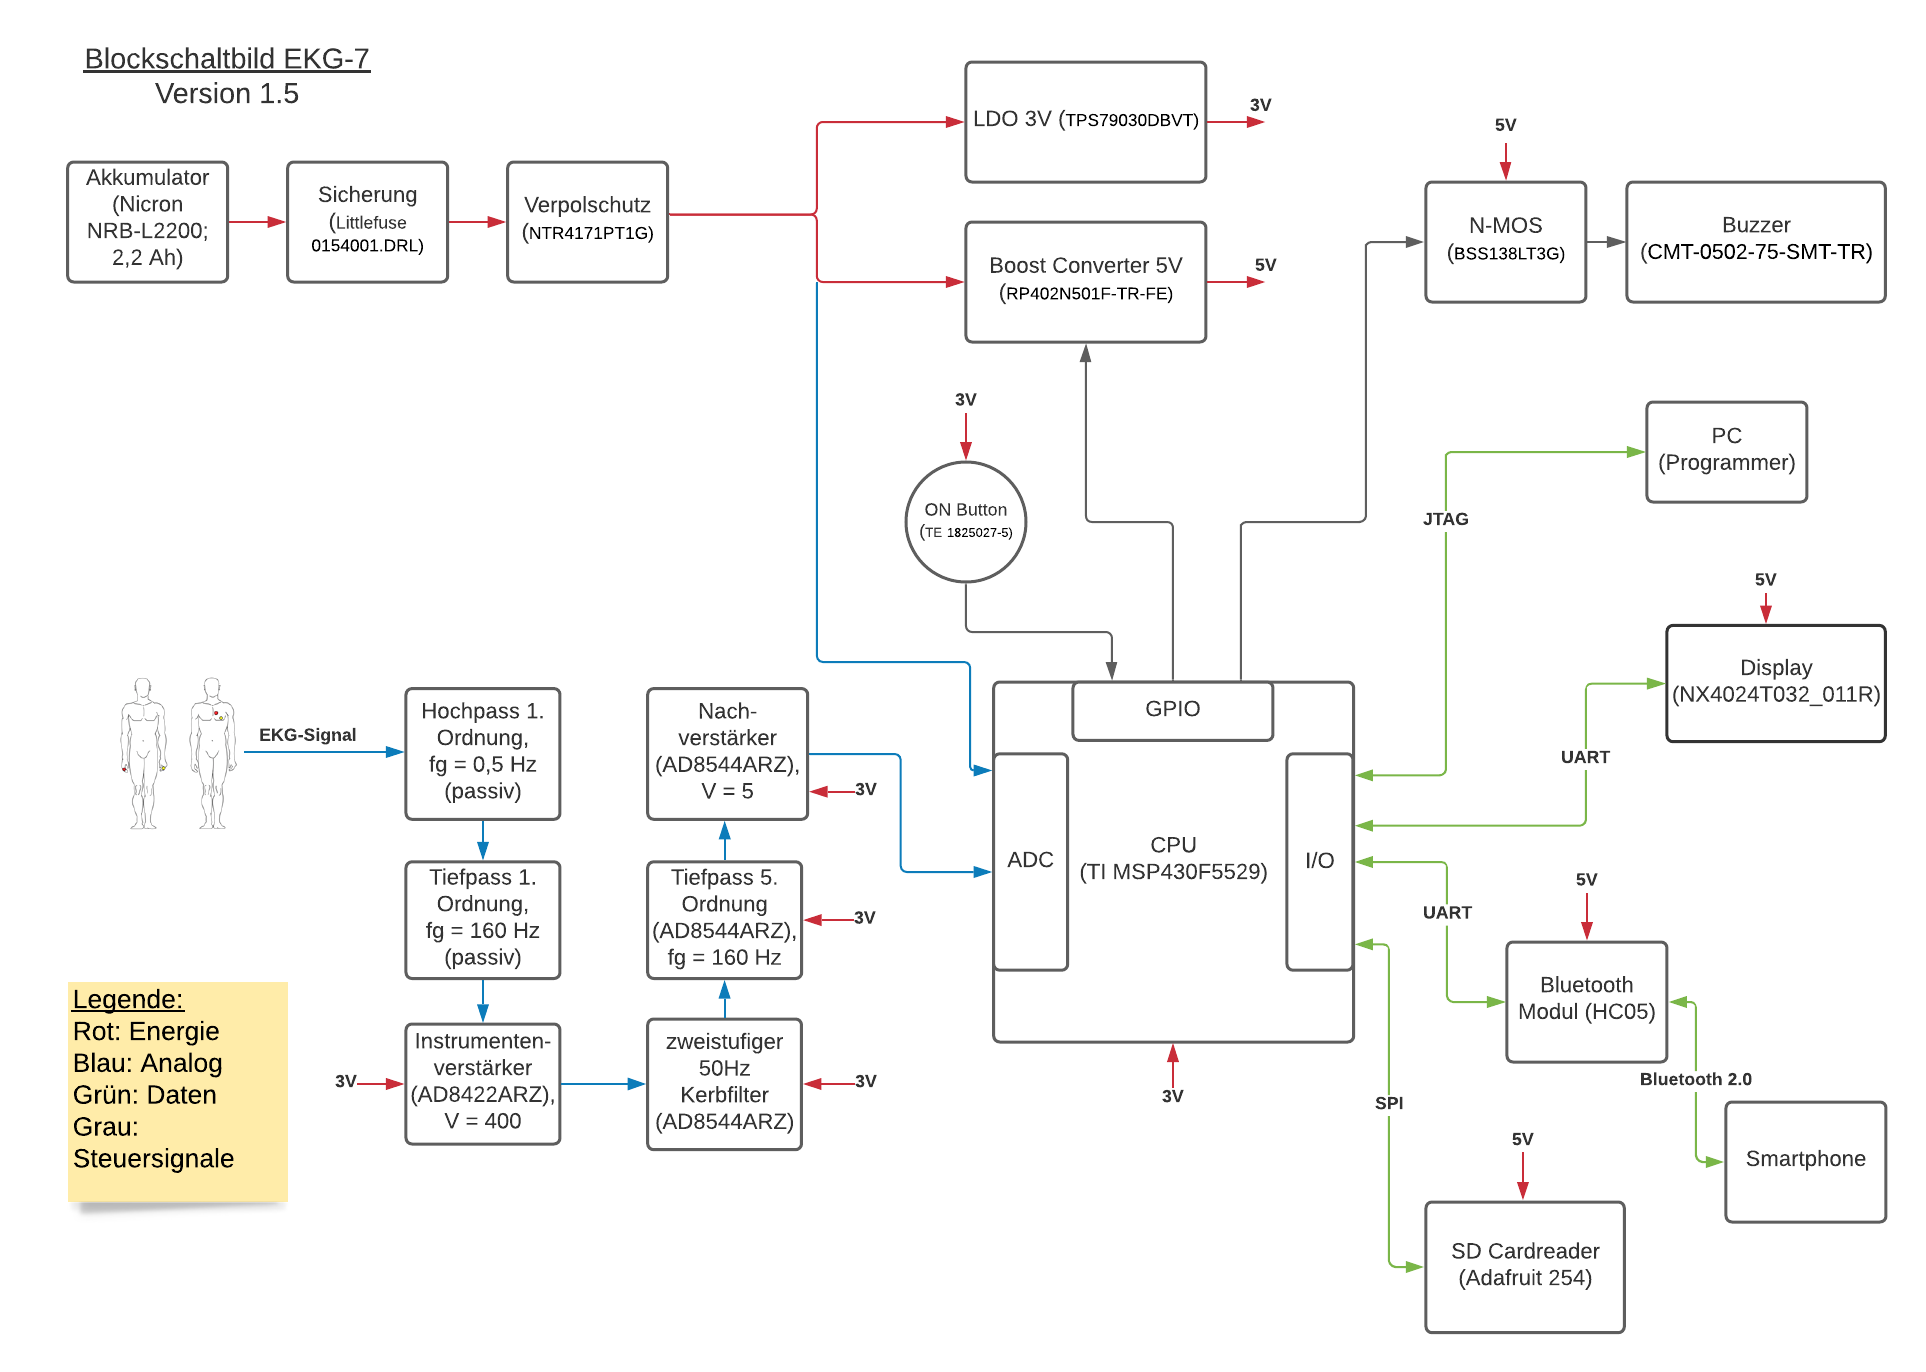
\includegraphics[width=\textwidth] {Blockschaltbild v1.5.png}
	\caption{Blockschaltbild des EKG-Geräts}
	\label{fig_Blockschaltbild} 
\end{figure}

%TODO PROJEKTGRUPPE: Konzeptionierung der jeweiligen Baugruppe  

\subsubsection{Verwendete Software}

Für die Erstellung und Frequenzanalyse eines künstlichen EKG-Signals wurde das numerische Rechentool Matlab verwendet. Damit konnten die Grenzfrequenzen des Signals bereits ohne Labortest abgeschätzt werden. Diese Erkenntnisse wurden bei der Schaltungsentwicklung der analogen Filterschaltung mit LTSpice angewandt. Durch die Einbindung von Herstellermodellen, war die Simulation von Bauteilen möglich, ohne diese physisch zu testen. Für den Entwurf der Leiterplatine kam Altium Designer zur Anwendung. Auch hierfür bieten Hersteller Modelle für die Pinbelegung, den Footprint und 3D-Modelle an. Besonders die 3D-Modelle waren für das Gehäusedesign hilfreich um die korrekte Lage und Maße der Bauteile im Gehäuse auch optisch zu prüfen.
%TODO PROJEKTGRUPPE: weitere Software die wir verwendet haben wie Blender, Nextion Editor, CCS, Git, etc...

\subsubsection{Verwendete Geräte}

\subsubsection{Bauteilbeschaffung und Fertigung} 

\subsubsection{Digitale Filterung}

Für die digitale Filterung des Netzbrummens wurden jeweils ein FIR- (Finite-Impuls-Response) und ein IIR- (Infinite-Impuls-Response) Filter als Bandsperren mit einer Sperrfrequenz von \SI{50} {\hertz} entworfen. Hierfür wurden die Filterkoeffizienten mit Matlab erzeugt und danach in C als eigenständige Module implementiert. Die Testung erfolgte auf dem Launchpad des MSP430 mit harmonischen Schwingungen zwischen \SI{1}{\hertz} und \SI{200}{\hertz}, einem künstlichen EKG-Signal (beides mit einer Signalquelle erzeugt) und einem echtem EKG-Signal. 

Der FIR-Filter verfügt zwar über einen linearen Phasenverlauf, erwies sich aber bei den Tests schnell als zu rechenintensiv, für die Anwendung auf dem verwendeten Prozessor. Mit ihm wurde bei einer Abtastfrequenz von \SI{250}{\hertz} lediglich eine Dämpfung von \SI{3}{\decibel} bis \SI{6}{decibel} erreicht.

Der IIR-Filter zeigte sich im Test mit verschiedenen harmonischen Schwingungen als sehr effizient mit einer maximalen Dämpfung von \SI{150}{\decibel} bei geringem Rechenaufwand. Jedoch führte er in der Anwendung bei einem echten EKG-Signal zu einer Verschlechterung des Ausgangssignals, da er Schwingungen erzeugte, wie aus Abbildung \ref{fig_Test_IIR_Filter} zu erkennen ist. 

\begin{figure} [h]
	%\centering
	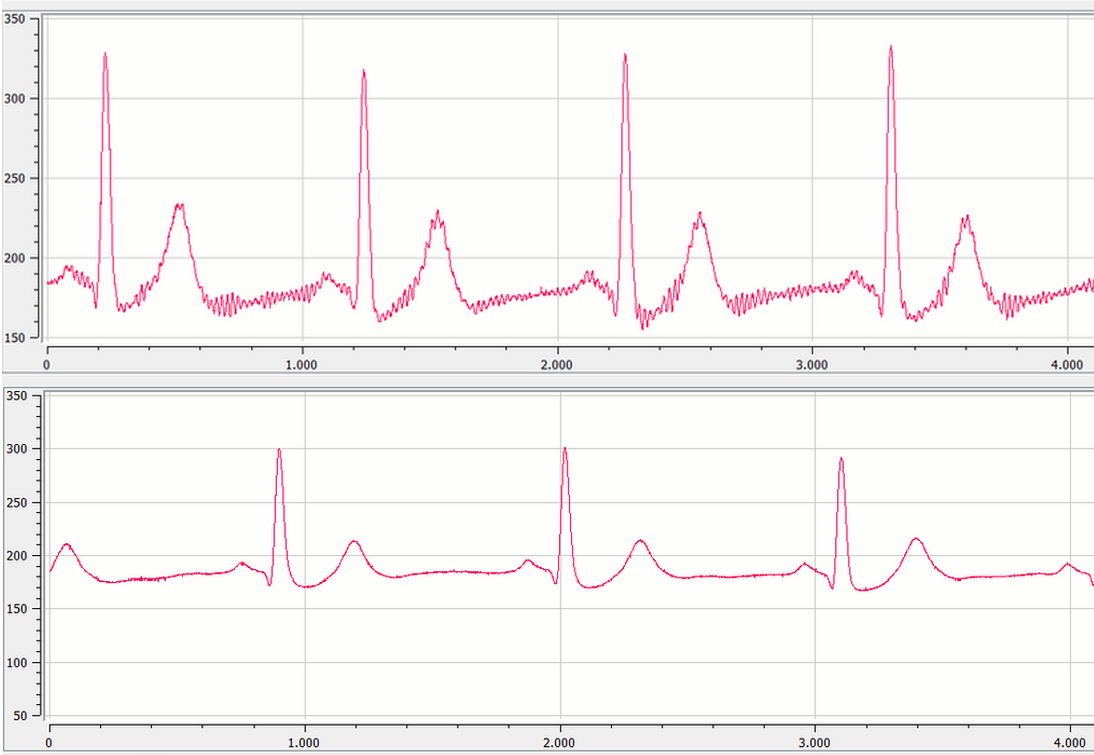
\includegraphics[width=\textwidth] {Test IIR Filter.png}
	\caption{oben: EKG-Signal mit durch IIR-Filter erzeugtes Störsignal; unten: EKG-Signal ohne IIR-Filterung}
	\label{fig_Test_IIR_Filter} 
\end{figure}
%TODO Anhang für FIR und IIR Filter



%TODO PROJEKTGRUPPE: weitere alternative Konzepte die wir ausprobiert oder in Betracht gezogen haben (zb. PMIC)